\documentclass[a4paper, 11pt]{report}
\usepackage[utf8]{inputenc}
\usepackage{amsmath,tabto}
\usepackage{hyperref}
\usepackage{titlesec}
\usepackage{graphicx}

\usepackage{glossaries}
\graphicspath{ {images/} }
\date{null}
\usepackage{fullpage} % changes the margin
\usepackage{setspace}
\begin{document}
\begin{titlepage} % Suppresses displaying the page number on the title page and the subsequent page counts as page 1
	\newcommand{\HRule}{\rule{\linewidth}{0.5mm}} % Defines a new command for horizontal lines, change thickness here
	
	\center % Centre everything on the page
	
	%------------------------------------------------
	%	Headings
	%------------------------------------------------
	
	\textsc{\LARGE Concordia University}\\[1.5cm] % Main heading such as the name of your university/college
	

	%------------------------------------------------
	%	Title
	%------------------------------------------------
	
	\HRule\\[0.4cm]
	
	{\huge\bfseries  SOEN 6481 - Software Systems Requirements Specification}\\[0.4cm] % Title of your document
	
	\HRule\\[1.5cm]
	\textsc{\Large Deliverable 1}\\[0.5cm] % Major heading such as course name
	\textsc{\Large Requirement Analysis for Ticket Vending Machine}\\[0.5cm]
	%------------------------------------------------
	%	Author(s)
	%------------------------------------------------
	
% 	\begin{minipage}{0.4\textwidth}
% 		\begin{flushleft}
			
% 			\end{flushleft}
% 	\end{minipage}
	~
% 	\begin{minipage}{0.4\textwidth}
% 		\begin{flushright}
			\large
			\textit{Supervisor}\\
			Prof. Pankaj Kamthan % Supervisor's name
% 		\end{flushright}
% 	\end{minipage}
    \vfill
    \large
            \textbf{Team A}\\
			\textit{Authors}\\
			Maria Ahmed - \textsc{40070844}\\
            Adarsh Aravind - \textsc{40082585}\\
            Sri Akhil Varma Alluri - \textsc{40082333}\\
            Dheeraj Ashok Shobha - \textsc{40082192}\\
            Charles Jebalitherson Augustin Moses - \textsc {40084105}\\
            
	
	% If you don't want a supervisor, uncomment the two lines below and comment the code above
	%{\large\textit{Author}}\\
	%John \textsc{Smith} % Your name
	
	%------------------------------------------------
	%	Date
	%------------------------------------------------
	
	\vfill\vfill\vfill\vfill% Position the date 3/4 down the remaining page
	\textbf{GitHub Address:} \url{https://github.com/charles-augustin/SOEN-6481}

	%------------------------------------------------
	%	Logo
	%------------------------------------------------
	
% 	\vfill\vfill
% 	
\includegraphics[width=0.2\textwidth]{download.png}\\[1cm] % Include a department/university logo - this will require the graphicx package
	 
	%----------------------------------------------------------------------------------------
	
	\vfill % Push the date up 1/4 of the remaining page
	
\end{titlepage}

%----------------------------------------------------------------------------------------


 
\tableofcontents
\chapter{Problem 1}
\section{Introduction}
In this document, we will analyze and discuss the online ticket vending machine that can be used in Montreal, Canada. The requirements and use cases are recorded in the pictorial representation with the help of problem domain, stakeholders and use case modeling to understand different perspectives of the system.
\section{Scope}
The online ticket vending machine(iGo) is used to serve public transportation including buses and local trains(metro). iGo users will have an online platform to recharge their OPUS cards and manage all the transactions in one place. iGo does not have any scope for maintaining the existing physical TVM's in metro stations.
\section{Description of iGo}
iGo is an online web application system where users can sign-up, login and recharge their OPUS cards. iGo will send all the data to STM's(Société de transport de Montréal) system through a secured communication protocol. iGo involves a variety of actors such as Government of Canada, Public Transport Authority(STM), Payment authority, customer, station master,etc. which makes it an interesting domain to study. \\\\
The traveler must sign up for an account with iGo for the first time or they can sign in as guest user where transaction history will not be available. For signing up into the system, it is mandatory to enter OPUS card number. Only one OPUS card can be linked per user to avoid internal complexities and fraudulent use of OPUS card. Once the user is logged into the system, user can recharge his/her opus card or purchase 1-way, 1-week, day or weekend pass based on the user's requirement. Users can also see their transaction history at any point in time to better understand the usability of iGo.\\\\
iGo will provide following services to its users,

\begin{enumerate}
    \item A customer must be able to sign-up to an online account with their email address or mobile number or any social media account (Google, Facebook) and be able to link their OPUS card to personal iGo account.
    \item A customer must be able to make payment in one of four ways namely Master/Visa debit card, Master/Visa credit card, iGo Wallet, Cash.
    \item A customer must be able to view their existing iGo wallet balance.
    \item A customer must be able to view their iGo transactions and must be able to print out their transactions.
    \item A customer must be able to schedule the pre-authorized payments for their OPUS cards.
    \item A customer must be able to add/ modify or delete personal information.
    \item A customer must be able to remove or add OPUS card from the iGo account at any point in time.
    \item A guest user must book tickets from the iGo by choosing appropriate ride options.
    \item All the users utilizing the iGo's in the metro station must be able to make payment with the cash and coins with maximum amount of \$80 per transaction.
\end{enumerate}

STM protects the customer information by handling the payments through high level secured communication protocol. iGo has in-built security feature to validate the card, here iGo initiates a request to connect with financial institutions. Once the connection is established, banking institution validates the given card against the PIN entered by the user. iGo has a strong established network that handles thousands of users on a daily basis and it is highly reliable.\\\\
iGo is also used to assist in the management of queue and priority of services in financial institutions, universities, and customer help desks of several organizations. It saves time, money and effort by providing the services in a quick and efficient manner. iGo is highly available but fails rarely due to power outage, internet service breakdown.\\\\
iGo will also maintain its internal log of transactions to resolve ambiguities arising from a connection failure in the middle of the transaction between iGo and STM System. Al the events will be recorded in the log when a traveler registers an account, logs in and also the web pages that user visits. This log data helps us to perform analytics and improve them to attract new customers.

\qquad\qquad\qquad\qquad \includegraphics[width=70mm,scale=0.5]
{opus.png}\\
\tab\tab\qquad\qquad Figure 1: A Sample OPUS card (Source: Carte OPUS)

\chapter{Problem 2}
\section{Context of use model : CU$_{I_{Go}}$}
\subsection{Users}
Users of iGo can be divided into registered and guest user, based on their reason to use the iGo. Users who will use iGo to buy ticket, pass or to recharge opus cards are registered users. Users who will use iGo to purchase tickets directly are guest users. Categories of different users are discussed in detail in the Classification and Tasks of users.
\begin{table}[ht]
    \centering
    \begin{tabular}{|l|l|}
    \hline
     \hline
    \multicolumn{2}{|l|}{Context of use factors}\\
      \hline
       \hline
    Type & Attribute  \\
     \hline
     User & Age, Residency, Education, Physical characteristics \\
      \hline
     User Role & Registered and Guest user \\
     \hline
      User Task & Buy tickets, passes, recharge card, development, maintenance  \\
       \hline
        User accessibility & Standing, On wheelchairs  \\
        \hline
        Technical Environment & Software, Screen, Keypad, Card readers, Cash collectors\\
        \hline
             Physical Environment & Dimension,Light  \\
               \hline
               Social Environment & Location, Space, User learn-ability, Privacy, Safety \& Security  \\ 
                \hline
              
                  \hline
              
    \end{tabular}
    \caption{Context of use factors}
    \label{tab:user}
\end{table}
\subsection{Classification and Tasks of Users}
\textsc{\large \bf Positive stakeholder} \newline
\textsc{\large \bf User:} User is A person who will use iGo to buy tickets, pass or to recharge OPUS card offered by STM. User is further divided into two categories: \\
Registered User: User who has an account in iGo web system.\\
Guest User: User who do not have an account in iGo web system.\\\\
\textsc{\large \bf User Characteristics:}\\
 Age: To buy a ticket or OPUS card, a user must be more than 10 years of age.\\
Proof of residency: To get a valid OPUS card from STM, a user must have a valid address in Quebec.\\
Education: It is assumed that the user will have the ability to read and understand either English or French language.\\
Physical Characteristics: The physical machine of iGo is accessible to all types of users. Users with wheelchair and impaired vision. iGo web page is accessible to colorblind users\\
\textsc{\large  Task:}\\ One can buy a one way, one-day tickets or weekly passes from the iGo using cash,coin or debit/credit card.\\
One can access the metro or bus using OPUS card given by STM too. A user can recharge his/her OPUS card from iGo. OPUS card users are allowed to have monthly recharge in advance for 3, 6 or 9 months. And, also they are allowed to recharge for next month in advance. \\\\
\textsc{\large  Constraints:} \\
Buying Opus card: Users can not buy OPUS card from iGo. They need to go to designated STM offices to buy OPUS card.\\
Using Cash: One user can not use more than \$80 cash in iGo at a time.\\\\
\textsc{\large \bf Station Master:}A person employed by STM who will be there to give any kind of assistance needed to use iGo. \\
\textsc{\large Task:} \\ They may help customers at the time of any kind of disruption of services, for example, if a valid service is not working they may assist by issuing the tickets or passes offered by iGo.They may assist a novice, differently-abled or aged user to learn how to use iGo. \\
\textsc{\large constraint:} \\Station Master must not disclose any critical information about iGo to negative stakeholders. \\\\
\textsc{\large \bf Development Team:} Team responsible for developing, testing, integrating or assembling the software or Hardware of iGo \\
\textsc{\large Task:}\\ The development team should have access to a valid requirement list for iGo. They should have required access to test the iGo application.\\
\textsc{\large Constraints:} \\
Known Publicly: Any member of development team including but not limited to project manager, developers, testers must not be known publicly.\\
Marketing purpose: The organization of the development team can not use any projects related to iGo for any kind of marketing or advertisement.\\\\
\textsc{\large \bf  Bank:} Canadian bank that processes all transactions of iGo.\\
\textsc{\large  Task:} Details of the banks that are involved in processing tasks of transactions are beyond the scope of iGo.\\\\
\textsc{\large \bf  Marketing Team:} Team dedicated to motivating people of Montreal to use iGo to access public transport. \\
\textsc{\large Task:} Marketing Team may use print media, broadcast media, internet to encourage end-users to use the service. They may offer any benefit or incentive to any users. \\
\textsc{\large constraint:}\\They are not allowed to give out any internal information. \\\\
\textsc{\large \bf Negative stakeholders}\\\\
\textsc{\large \bf  Hacker:} \\
\textsc{\large  Task:}Hacker may abuse any software or hardware to get information either from iGo or personal information of users.\\\\
\textsc{\large \bf  Competitor:}\\
\textsc{\large  Task:}Competitor may get any internal information of iGo to come up with a new improved version.
\subsection{Environment:}
\large{\textbf{Technical Environment}}\\
\large{\textbf{Software:} The iGo website should be accessible from any desktop, laptop or mobile device.  \\
\textsc{\large \bf Screen:}   \\
\textsc{\large Task:}Screen of the physical machine in the metro station should be accessible by both touch and buttons. The web page of iGo should be accessible for color-blind users. \\
\textsc{\large constraint:} To offer better usability, the screen should not contain more than four items at a time.\\
\textsc{\large \bf Keypad:} \\
\textsc{\large Task:} In physical iGo the keypad must be inclined such a way that it is accessible to people irrespective of their physical disabilities. Buttons must support braille. Different buttons should have a different sound to help to distinguish among different keystrokes. \\
\textsc{\large \bf Payment Card Reader:} \\
\textsc{\large Task:} Payment card reader should have the capability to read all Canadian bank cards and it should be positioned in such a way that gives the highest privacy to users.   \\
\textsc{\large \bf Opus Card Reader:} \\
\textsc{\large Task:} Opus card reader should have the capability to recognize valid opus cards.  \\
\textsc{\large \bf  Cash Dispenser:}\\
\textsc{\large Task:} User can buy tickets, pass or recharge opus card using cash or coin from the iGo in a metro station. \\\\
\textsc{\large \bf Physical Environment}\\
\textsc{\large \bf Dimension:} Height of the physical machine should be such that it's accessible by all users irrespective of height. \\
\textsc{\large \bf Light:} Light should be adequate so that users can clearly see the screen, keypad, and different cardholders. \\\\
\textsc{\large \bf Social Environment}\\
\textsc{\large \bf Location:} The machine should be placed near the station masters booth and close to the mechanical gates of the metro. The physical machine should be protected from any extreme weather conditions such as rain or snow. \\
\textsc{\large \bf Space:} There must be adequate space in front of the physical iGo so that a minimum of 10 people can line up in front of it. \\
\textsc{\large \bf  Instructions to novice users:} The website of iGo should have a proper video demonstrating the use of the system for different users.\\
\chapter{Problem 3}
 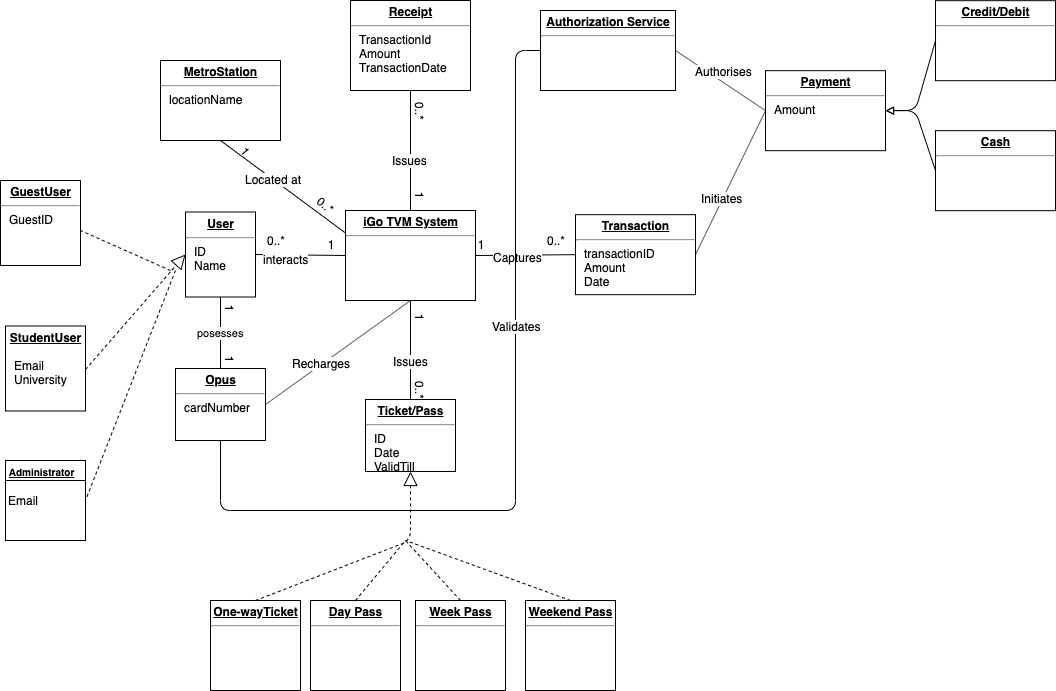
\includegraphics[width=180mm,height=150mm,scale=0.5]
{DomainDiagram.jpg}

\tab\tab\qquad\qquad\qquad\qquad\qquad Figure 2: Domain model for iGo\\
\\
\\
\textsc{\large{\bf{Domain Model: DM$_{I_{GO}}$ } }}\\\\ The Domain model above captures all the real-world concepts that are involved in the iGo. The model expresses the relationship with each class and also the multiplicity of how they are connected. The users have been made as an abstract class that will be implemented by the GuestUser, RegisteredUser.
Also, the Ticket/pass has been shown as an abstract class. Payment is considered as an abstract class with some common methods that can be further overridden by Credit/Debit and cash classes' methods.
\\\\
One instance of an iGo TVM can issue zero or more tickets and zero or more receipts, it can interact with zero or more users. Multiple instances iGo can be located at one instance of a metro station depending on the requirement as per the expected number of daily users, minimum being one iGo per station. iGo captures zero or more transactions created by the users.
\\
The transaction history domain class has a composition relationship with the transaction as it holds the list of all transactions for a particular user and those transactions can't be a part of another user's transaction history.
\\
The user is an abstract class and Guest user and Registered user are the two types of users. Every registered user can have zero or one instance of an opus card that will be recharged by the iGo. The card is validated by the authorization service when it is linked with the user account. The Guest user can directly purchase the ticket /pass without having an account or an opus card.
\\
The Ticket/Pass class has the common attributes i.e ID, date of issue and Valid Till. It has 4 child classes, One-way ticket, weekend pass, weekly pass, day pass. Both the registered user and guest user can purchase any of these tickets. Hence the relation from the user abstract class to the ticket abstract class has been shown. 
\\
A transaction initiates a payment that can be either Cash or Credit/Debit. Each payment will be authorized by the bank authorization service.
\chapter{Problem 4}
\section{Use case model: UCM$_{I_{GO}}$}
 \includegraphics[width=165mm,height=150mm,scale=0.5]
{UseCaseModel.jpg}

\tab\tab\qquad\qquad\qquad\qquad\qquad\qquad\qquad Figure 3: Use case Model for iGo\\\\
In this use case model, there are 5 actors namely User, Registered user, Guest user, Admin, and Bank. User is an abstract actor which is implemented by Registered user and Guest user. For the first-time use, the user will have to sign up into an iGo account with his/her email address. iGo will store the user credentials in the database. There will be an alert message if the email is invalid. After signing in, users can link their OPUS card with their iGo account. Admin will authenticate OPUS card.\\\\ Registered user should log in to his/her account on iGo website. There will be an alert message displayed by iGo if the credentials don’t match. Users can purchase a ticket either at the station or through the iGo website by selecting from the categories available. Purchase ticket use case consists of various ticket types from which the user can select one. User can recharge the card either with the TVM or through the iGo website. \\\\ If user wants to recharge online he/she can do it at anytime. Pre-authorized payments are also given as an option to an user. User can remove their opus card from their account at any point of time and also delete his/her account. Payments at STM stations can be completed through a Debit/Credit card. Coins/Bills can also be used. This information is secured by STM using security APIs. Users can keep track of their transaction history for their reference. There is an option to print their records also. Users can check their iGo wallet balance once they login to their account and they can reload the wallet whenever they wish to.


\section{Sequence Diagram}
\subsection{Positive Use Cases}
\large{\textbf{Recharge opus}}\\
Below sequence diagram captures the interaction between the actor, iGo and subsystem: cash dispenser and a tertiary actor i.e the bank. It shows the positive flows when the user has to recharge his opus card. The diagram depicts the different payment options that are available to the user.\\
The user logs into the iGo using his credentials and he will choose the option to recharge his opus card. He will select one of the available payment options either Credit/Debit or Cash. If its Credit/Debit the user will insert his card to the card reader and also enter the PIN. Then the transaction details are sent to the Bank. The bank authorizes the transaction and a receipt is printed out for the user. If he selects the Cash option he can drop in the cash in the dispenser and the dispenser validates the amount to check if it's the right amount and a receipt will be issued if that's the case along with differential amount as change.\\
 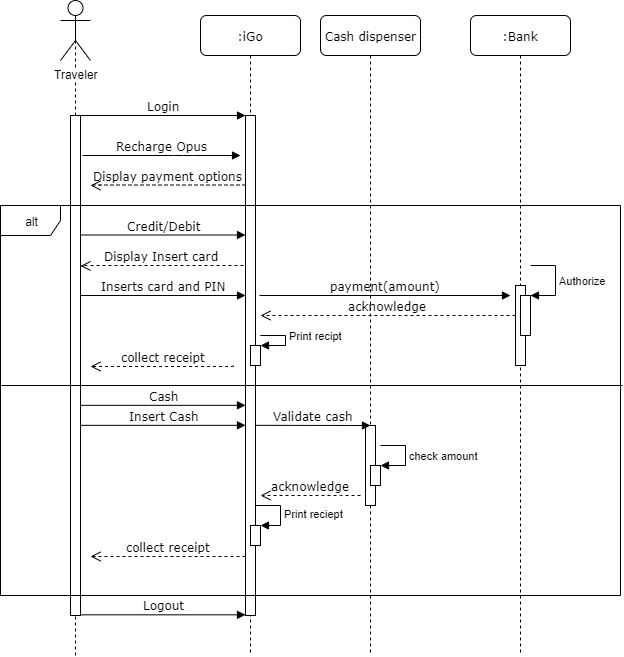
\includegraphics[width=150mm,height=150mm,scale=0.5]
{SequenceDiagram_Recharge.jpg}

\tab\tab\qquad\qquad\qquad\qquad
Figure 4: Sequence diagram - Recharge Scenario \\\\
\large{\textbf{Buy Ticket/Pass}}\\
The below sequence diagram captures the interaction between the actor, iGo and subsystem; a cash dispenser and a tertiary actor i.e the bank as the above diagram. It shows the positive flows when the user has to buy a one-way ticket or Day/Week/Weekend pass. The system handles the different payment options available to the user.\\\\
The user logs into the iGo using his credentials and he will choose the option to buy pass/ticket then options will be displayed to select the type of pass or ticket. He will select one of the options and proceed to pay with the same steps as described in the above diagram.

 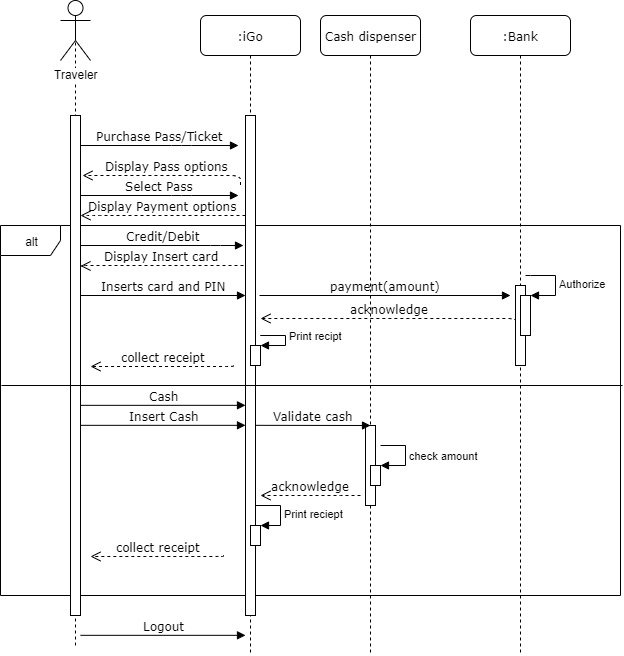
\includegraphics[width=150mm,height=150mm,scale=0.5]
{SequenceDiagram_Pass.jpg}\\
\tab\tab\qquad\qquad\qquad\qquad
Figure 5: Sequence diagram - Pass Scenario \\\\
\large{\textbf{Viewing Transaction History}}\\\\
Under the positive use case, let us consider the user tries to view the transaction history in iGo account. The iGo system records the history of all the transactions performed by registered user. As a first step, user logs into iGo System, if user is authenticated, iGo will show the linked OPUS card. User can then select the linked OPUS card to request the view of transaction history. iGo provides a view of all the transactions. From the view, user can select a particular transaction to view its details such as the date, mode of payment if any. After this, user can request to print transaction history, iGo will handle it internally and prints the paper to the customer. The customer logs out from the system to end the transaction.\\\\

\qquad\qquad\qquad\qquad
 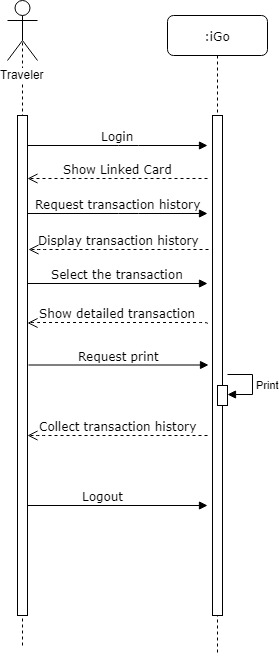
\includegraphics[width=78mm,height=150mm,scale=0.5]
{Sequence_Transaction_History.jpg}\\
\tab \qquad \quad\qquad Figure 6: Sequence diagram for viewing transaction history
\section{Activity Diagram: AD$_{I_{GO}}$}
 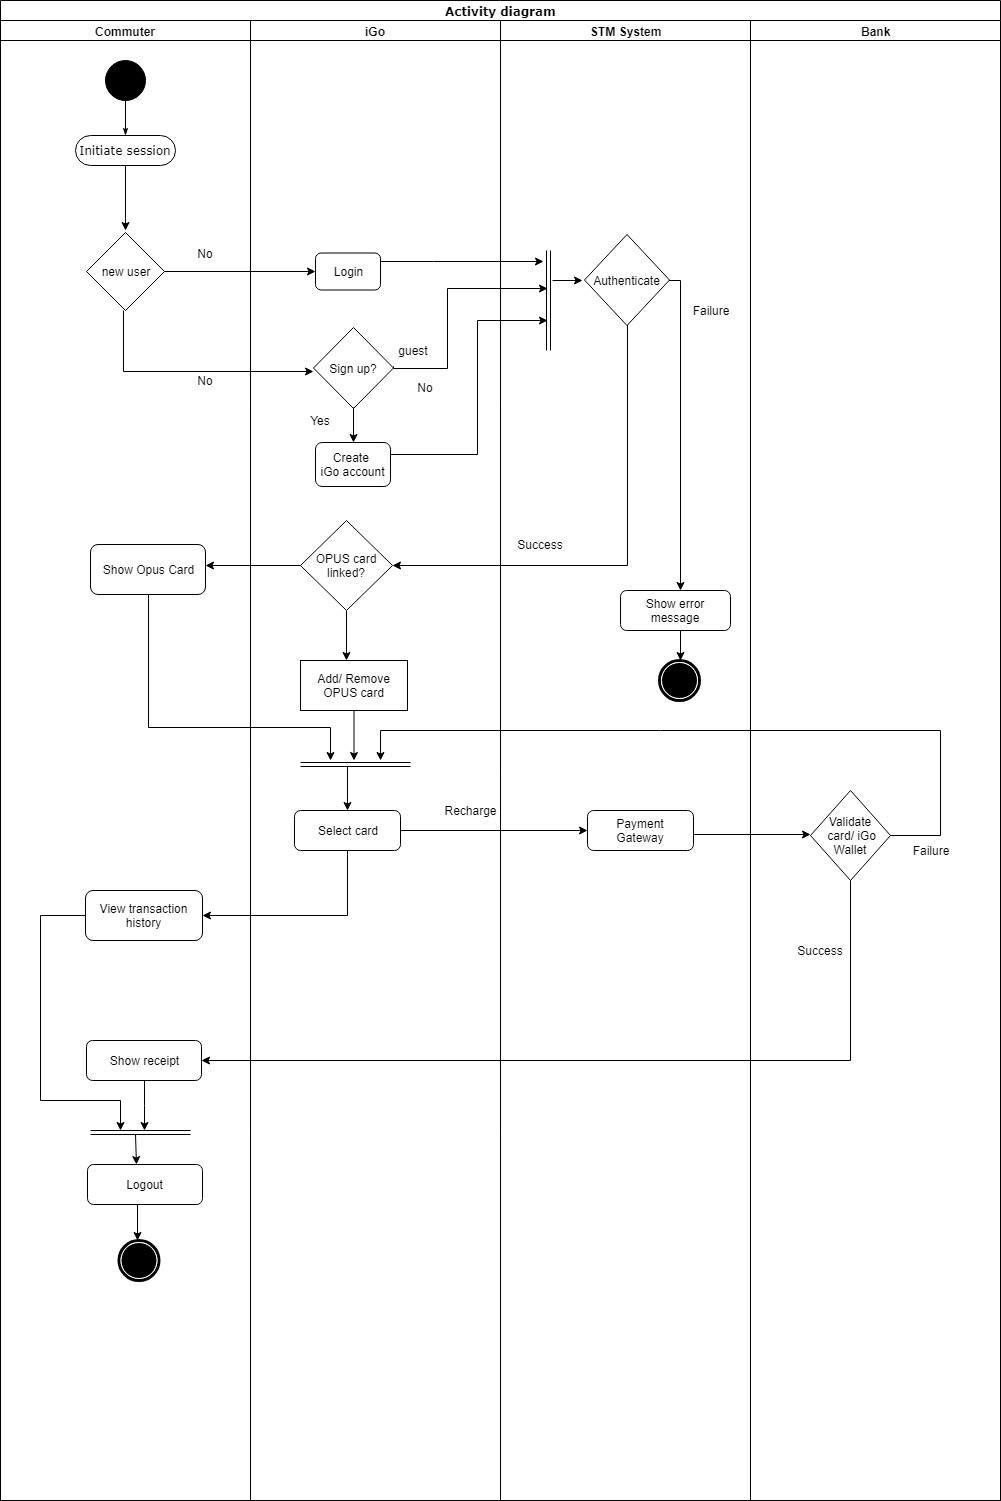
\includegraphics[width=161mm,height=220mm,scale=0.5]
 {Activity_Diagram.jpg}\\
\tab\tab\qquad\quad\qquad\qquad\qquad Figure 7: Activity Diagram (AD$_{I_{GO}}$)
\section{Negative Use Cases}
 \large{\textbf{System Overload}}\\
 Since iGo is a public service application, there will be millions of users accessing the system at a time. Hence, iGo application server must have the capability to service requests without system flooding problems. \\\\
 \large{\textbf{Security vulnerability - Hacker}}\\
 In today's world, there is a high possibility of malware attack to steal the customer information, Hence, iGo should perform all the transaction through secured communication layer that prevents the intruders from getting into the system to steal confidential data.\\\\
 \large{\textbf{Preventive measure}}\\
 Using security modeling tools such as Sea Monster (source: lecture notes), Microsoft threat modelling tool, we can prevent the system flooding, hackers and other misusers from attacking the system. \\\\
 \large{\textbf{Exception Scenarios}}\\\\
 \large{\textbf{Authentication Failure}}\\
 When the user tries to login with invalid email address or password, iGo will handle it appropriately and displays a proper error message to the user.\\\\
 \large{\textbf{Payment Failure}}\\
 When the user enters an invalid card such as card number, CVV or card has expired on a given date or not enough money in the wallet, iGo must be designed in such a way to handle all these exceptions.\\\\
 \large{\textbf{Expired OPUS Card}}\\
 If the linked OPUS card expires in the future and the customer performs a transaction with an expired card, transaction will fail. Hence, the customer should get notification in advance (at least 1 month) about the card expiration.
\chapter{Glossary}
 \begin{itemize}
\item iGo - iGo	The online Ticket Vending Machine Web Application.
\item Positive Stakeholder- Stakeholder who wants to contributes to the project in a positive manner.
\item Negative Stakeholder- Stakeholder who wants to harm the project or wants to contribute in a negative manner.
\item OPUS - OPUS is the name of STM traveling card which is used by people to travel by the STM metro, manufactured and distributed by STM agencies.
\item CU$_{I_{GO}}$ - Context of use model for iGo.
\item DM$_{I_{GO}}$ - DM$_{I_{GO}}$	Domain model representation for iGo.
\item UCM$_{I_{GO}}$ - Use Case modeling for iGo.
\item AD$_{I_{GO}}$ - Activity Diagram for iGo.
\item TVM - Ticket Vending Machine
\item STM - Société de transport de Montréal public transportation company.
\end{itemize}
\chapter{Tools Used}
 \begin{itemize}
     \item Overleaf
     \item Draw.io
     \item GitHub
     \item Git wiki
     \item Google forms/drive
 \end{itemize}
\chapter{References}
\begin{enumerate}
  \item \url{http://www.stm.info/en}
  \item PANKAJ KAMTHAN (2019) “Understanding Context"
  \item PANKAJ KAMTHAN (2019) “Introduction to Interviews”
  \item PANKAJ KAMTHAN (2019) “Introduction To Domain Modeling” - Section 14, 15 ,16.
  \item PANKAJ KAMTHAN (2019) “Introduction To Use Case Modeling” - Section 11, 12.
  \item PANKAJ KAMTHAN (2019) “Negative Use Case Modeling”  - Section 8
  \item \url{https://www.lucidchart.com/pages/uml-activity-diagram}
  \item Carte OPUS. To obtain your photo OPUS card. 2019. \url{http://www.carteopus.info/}.
\end{enumerate}

\chapter{Appendix}
\textbf{\LARGE{Interview Questions}}\\\\
\textbf{Interview 1:}\\\\
Date – 23-09-2019, 5:45 PM\\
Interviewers – Maria, Akhil\\
Interviewee – Krishnan Krishnamurthy \\\\
Question – Are you a current worker or retired from STM?\\
Answer – No\\\\
Question – Age (10-20, 20-40, 40-60, 60-80, 80-100)\\
Answer – 20-40\\\\
Question – Gender (Female, Male, Prefer not to say)\\
Answer – Male\\\\
Question – What public transportation do you use the most? (Metro, Bus, Both)\\
Answer – Both.\\\\
Question – Have you used TVM before? (No, Yes)\\
Answer 1 – Yes\\\\
Question – If yes, what difficulties have you faced during the transaction?\\
Answer – Waiting in queue every month while recharging my OPUS card.\\\\
Question – If you are using the machine for the first time, how important is the demo video or a set of instructions to operate the machine? (0-5 scale, 0 being least important and 5 being most important)\\
Answer – 3\\\\
Question – Have you used TVM at the same station or different stations? (Same Station, Different Stations)\\
Answer – Different Stations\\\\
Question – If you have used the machine at multiple stations, what differences did you notice?\\
Answer – They are almost the same\\\\
Question – Which machine do you consider the best? And why?\\
Answer – None\\\\
Question – Select the category of differently abled people for whom current TVM gives enough accessibility. (Blindness, Color Blindness, Disability to walk, All of the above, None of the above)\\
Answer – Disability to walk\\\\
Question – Would you like to have TVMs at selected bus stops as well? (Yes, No, Maybe)
Answer – Yes\\\\
Question – What type of pass do you purchase the most? (Daily, Weekly, Monthly, One way, Two way)\\
Answer – Monthly\\\\
Question – What specific ticket type would you like to be offered? (Paper ticket, E-Ticket)\\
Answer – E-Ticket\\\\
Question – If you are a monthly subscriber to STM, do you recharge on the first day of every month? (Yes, No, Maybe)\\
Answer – Yes\\\\
Question – What are the other means of transport you use? \\ 
Answer – Car\\\\
Question – Is the screen light in TVM adequate to perform any transaction? (Yes, No, Maybe)\\
Answer – Yes\\\\
Question – What kind of interface do you prefer at the TVM? (Button operated, Touch screen, Both)\\
Answer – Both\\\\
Question – Is the screen accessible for people with the color vision deficiency? (Yes, No, Maybe)\\
Answer – Yes\\\\
Question – Ease of access (0-5 scale)\\
Answer – 3\\\\
Question – What is your convenient method to make a payment? (Cash, Online, Debit/Credit)\\
Answer – Debit/Credit\\\\
Question – As a frequent user, do you prefer to buy the printed ticket or to reload your OPUS card? (Printed ticker, Reload OPUS card)\\
Answer – Reload OPUS card\\\\
Question – Which kind of payment receipt will be more convenient for you? (Paper receipt, e-receipt)\\
Answer – Paper receipt\\\\
Question – Would you prefer an online application to perform all the transactions related to TVM at one place? (Yes, No, Maybe)\\
Answer – Yes\\\\
Question – Which language do you prefer other than English and French when using the TVM system?
Answer – None\\\\
Question – Would like to see Tap-to-pay option to the current TVM? (Yes, No, Maybe)\\
Answer – Yes\\\\
Question – Do you prefer to hear the process as guidance? (Yes, No, Maybe)\\
Answer – Maybe\\\\
Question – Would you prefer to have a monthly subscription for your pass where your card will be recharged automatically at the first of every month? (Yes, No)\\
Answer – Yes\\\\
Question – Would you like to recharge your card before 1st of every month manually? (Yes, No, Maybe)\\
Answer – Maybe\\\\
Question – Do you have any other improvements to be included?\\
Answer – Payment options should include tap to pay\\\\
\textbf{Interview 2:}\\\\
Date – 25-09-2019, 11:00 AM \\
Interviewers – Adarsh, Dheeraj\\
Interviewee – Darwin \\\\
Question – Are you a current worker or retired from STM?\\
Answer – No\\\\
Question – Age (10-20, 20-40, 40-60, 60-80, 80-100)\\
Answer – 20-40\\\\
Question – Gender (Female, Male, Prefer not to say)\\
Answer – Male\\\\
Question – What public transportation do you use the most? (Metro, Bus, Both)\\
Answer – Both.\\\\
Question – Have you used TVM before? (No, Yes)\\
Answer – Yes\\\\
Question – If yes, what difficulties have you faced during the transaction?\\
Answer – Long queue, Confusing interface, and card was not working, there was no other option to pay. \\\\
Question – If you are using the machine for the first time, how important is the demo video or a set of instructions to operate the machine? (0-5 scale, 0 being least important and 5 being most important)\\
Answer – 4\\\\
Question – Have you used TVM at the same station or different stations? (Same Station, Different Stations)\\
Answer – Different Stations\\\\
Question – If you have used the machine at multiple stations, what differences did you notice?
Answer – Some has better lighting\\\\
Question – Which machine do you consider the best? And why?\\
Answer – Guy Concordia, cause there's lots of space to line up\\\\
Question – Select the category of differently abled people for whom current TVM gives enough accessibility. (Blindness, Color Blindness, Disability to walk, All of the above, None of the above)\\
Answer – Disability to walk\\\\
Question – Would you like to have TVMs at selected bus stops as well? (Yes, No, Maybe)\\
Answer – Yes\\\\
Question – What type of pass do you purchase the most? (Daily, Weekly, Monthly, One way, Two way)\\
Answer – Monthly\\\\
Question – What specific ticket type would you like to be offered? (Paper ticket, E-Ticket)\\
Answer – E-Ticket\\\\
Question – If you are a monthly subscriber to STM, do you recharge on the first day of every month? (Yes, No, Maybe)\\
Answer – Yes\\\\
Question – What are the other means of transport you use?  \\
Answer – Bus\\\\
Question – Is the screen light in TVM adequate to perform any transaction? (Yes, No, Maybe)\\
Answer – Yes\\\\
Question – What kind of interface do you prefer at the TVM? (Button operated, Touch screen, Both)\\
Answer – Both\\\\
Question – Is the screen accessible for people with the color vision deficiency? (Yes, No, Maybe)\\
Answer – Maybe\\\\
Question – Ease of access (0-5 scale)\\
Answer – 2\\\\
Question – What is your convenient method to make a payment? (Cash, Online, Debit/Credit)\\
Answer – Online\\\\
Question – As a frequent user, do you prefer to buy the printed ticket or to reload your OPUS card? (Printed ticker, Reload OPUS card)\\
Answer – Reload OPUS card\\\\
Question – Which kind of payment receipt will be more convenient for you? (Paper receipt, e-receipt)\\
Answer – e-receipt\\\\
Question – Would you prefer an online application to perform all the transactions related to TVM at one place? (Yes, No, Maybe)\\
Answer – Yes\\\\
Question – Which language do you prefer other than English and French when using the TVM system?\\
Answer – None\\\\
Question – Would like to see Tap-to-pay option to the current TVM? (Yes, No, Maybe)\\
Answer – Yes\\\\
Question – Do you prefer to hear the process as guidance? (Yes, No, Maybe)\\
Answer – Maybe\\\\
Question – Would you prefer to have a monthly subscription for your pass where your card will be recharged automatically at the first of every month? (Yes, No)\\
Answer – Yes\\\\
Question – Would you like to recharge your card before 1st of every month manually? (Yes, No, Maybe)\\
Answer – Maybe\\\\
Question – Do you have any other improvements to be included?\\
Answer – Pre-authorized payment option to recharge OPUS card\\\\
\textbf{Interview 3:}\\\\
Date – 29-09-2019, 12:50 PM \\
Interviewers – Charles, Adarsh\\
Interviewee – Riya \\\\
Question – Are you a current worker or retired from STM?\\
Answer – No\\\\\\
Question – Age (10-20, 20-40, 40-60, 60-80, 80-100)\\
Answer – 40-60\\\\
Question – Gender (Female, Male, Prefer not to say)\\
Answer – Female\\
Question – What public transportation do you use the most? (Metro, Bus, Both)\\
Answer – Metro.\\\\
Question – Have you used TVM before? (No, Yes)\\
Answer 1 – Yes\\\\
Question – If yes, what difficulties have you faced during the transaction?\\
Answer – No. \\\\
Question – If you are using the machine for the first time, how important is the demo video or a set of instructions to operate the machine? (0-5 scale, 0 being least important and 5 being most important)\\
Answer – 2\\\\
Question – Have you used TVM at the same station or different stations? (Same Station, Different Stations)\\
Answer – Different Stations\\\\
Question – If you have used the machine at multiple stations, what differences did you notice?
Answer – None\\\\
Question – Which machine do you consider the best? And why?\\
Answer – None\\\\
Question – Select the category of differently abled people for whom current TVM gives enough accessibility. (Blindness, Color Blindness, Disability to walk, All of the above, None of the above)\\
Answer – None of the above\\\\
Question – Would you like to have TVMs at selected bus stops as well? (Yes, No, Maybe)\\
Answer – Maybe\\\\
Question – What type of pass do you purchase the most? (Daily, Weekly, Monthly, One way, Two way)\\
Answer – Monthly\\\\
Question – What specific ticket type would you like to be offered? (Paper ticket, E-Ticket)\\
Answer – E-Ticket\\\\
Question – If you are a monthly subscriber to STM, do you recharge on the first day of every month? (Yes, No, Maybe)\\
Answer – Yes\\\\
Question – What are the other means of transport you use? \\ 
Answer – Bus\\\\
Question – Is the screen light in TVM adequate to perform any transaction? (Yes, No, Maybe)\\
Answer – Yes\\\\
Question – What kind of interface do you prefer at the TVM? (Button operated, Touch screen, Both)\\
Answer – Touch screen\\\\
Question – Is the screen accessible for people with the color vision deficiency? (Yes, No, Maybe)\\
Answer – Maybe\\\\
Question – Ease of access (0-5 scale)\\
Answer – 5\\\\
Question – What is your convenient method to make a payment? (Cash, Online, Debit/Credit)\\
Answer – Online\\\\
Question – As a frequent user, do you prefer to buy the printed ticket or to reload your OPUS card? (Printed ticker, Reload OPUS card)\\
Answer – Reload OPUS card\\\\
Question – Which kind of payment receipt will be more convenient for you? (Paper receipt, e-receipt)\\
Answer – e-receipt\\\\
Question – Would you prefer an online application to perform all the transactions related to TVM at one place? (Yes, No, Maybe)\\
Answer – Yes\\\\
Question – Which language do you prefer other than English and French when using the TVM system?\\
Answer – None\\\\
Question – Would like to see Tap-to-pay option to the current TVM? (Yes, No, Maybe)\\
Answer – Maybe\\\\
Question – Do you prefer to hear the process as guidance? (Yes, No, Maybe)\\
Answer – Yes\\\\
Question – Would you prefer to have a monthly subscription for your pass where your card will be recharged automatically at the first of every month? (Yes, No)\\
Answer – Yes\\\\
Question – Would you like to recharge your card before 1st of every month manually? (Yes, No, Maybe)\\
Answer – Yes\\\\
Question – Do you have any other improvements to be included?\\
Answer – Increase processing speed.\\
\end{document}
